% http://pgfplots.net/media/tikz/examples/TEX/intersection-surfaces.tex
% +3d+pgf
% compile with lualatex
%
\documentclass[border=10pt]{standalone}
%%%<
\usepackage{verbatim}
%%%>
\usepackage{pgfplots}
\pgfplotsset{width=7cm,compat=1.8}

\begin{comment}
:Title: Intersection of two surfaces
:Tags: 3D;Intersections
:Author: Jake
:Slug: intersection-surfaces

We would like to intersect a 3D plot with a plane. The problem is not to get
the two functions into a plot, but to get the two functions to visual
intersect with each other, i.e the nearest surface is in the foreground.

This can't be done automatically, unfortunately, since pgfplots can't do z
buffering between different \addplot commands.

For this concrete application, you could construct the plot "by hand", however:

First, you draw the part of the cone below 0, then you draw the plane and the
circle, then you draw the part of the cone above 0.

I've used a polar coordinate system for this, since it makes the input of
polar functions easier.

This code was written by Jake on TeX.SE.
\end{comment}

\begin{document}
  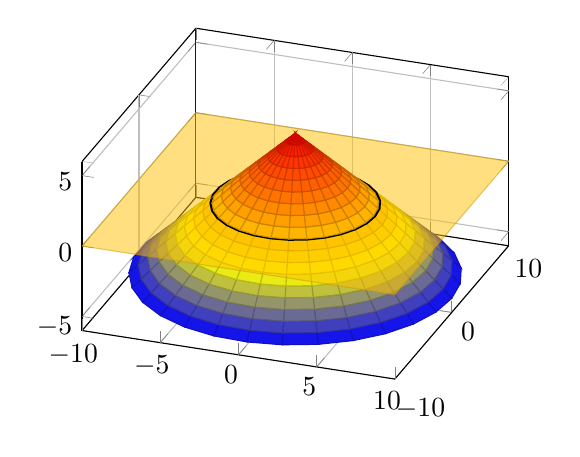
\begin{tikzpicture}
    \begin{axis}[grid=major,view={20}{40},z buffer=sort, data cs=polar]
      \addplot3 [surf, domain=0:360, domain y=5:10,samples=30, samples y=10]
      {-y+5};
      \addplot3 [data cs=cart,surf,domain=-10:10,samples=2, opacity=0.5]
      {0};
      \addplot3 [domain=0:360, samples y=0, samples=30, thick, z buffer=auto]
      (x,5.1,0);
      \addplot3 [surf,domain=0:360, domain y=0:5,samples=30, samples y=10]
      {-y+5};
    \end{axis}
  \end{tikzpicture}  
\end{document}